\chapter{Introduction}
\label{:intro}

Range searching is one of the most common types of problems which arise in everyday computer use. 
With a range search, we are given a set of objects and asked to identify those which satisfy some bounded criteria. 
Range searches can take many different forms: searching for email received between two dates, looking for restaurants near your present location, or identifying what a video game player should see on their screen in any one frame; these are all examples of range searches.

In computational geometry, range searching takes on a more abstract quality. 
Typically we are given an environment containing a set of geometric objects such as points, lines, circles, or boxes. 
A query is itself another well-defined geometric object, and our goal is to identify all elements of the environment contained within the query region.  
When addressing a range searching problem, we want to develop a method for preprocessing the input environment so that we can answer any query as efficiently as possible.
Given how common and flexible range searching is to such a wide range of practical computer science, it is not surprising to find that a great deal of research has been expended in this area.  

In this thesis, we address the notion of \emph{Partial Enclosure Range Searching (\PERS{})}, which, to the best of our knowledge, has not been explored previously. 
In this setting, our goal is to identify, for a given query region, all objects which satisfy the \emph{Partial Enclosure Property}, which specifies that an object must intersect a query region by at least some fixed proportion of the object's own size (e.g., length, area, volume) in order to be selected.

This chapter is organized as follows.
Section~\ref{:intro:motivation} begins by describing our motivation for this problem. 
In Section~\ref{:intro:problems} we describe the specific variations of the \PERS{} problem that we will address in this thesis. 
In Section~\ref{:intro:related}, we discuss related problem domains, and contrast them to our own.
Section~\ref{:intro:contributions} outlines the contributions made by this thesis.
We conclude the introduction by outlining the organization of the remainder of the thesis in Section~\ref{:intro:organization}.


%------------------------------------------------------------------------------
%------------------------------------------------------------------------------
\section{Motivation}
\label{:intro:motivation}

This problem was inspired by the author's use of Microsoft OneNote. 
Using a digital pen, OneNote can be used much like a paper notebook, allowing the user to add handwriting, diagrams, equations, and any other such thing to a page.
Unlike a paper notebook, OneNote also allows the user to select previously drawn objects in order to translate, scale, copy and otherwise manipulate them.
Figure~\ref{fig:intro:onenote} shows some handwritten notes, and a diagram which has been partially selected.

\begin{figure}
\begin{center}
  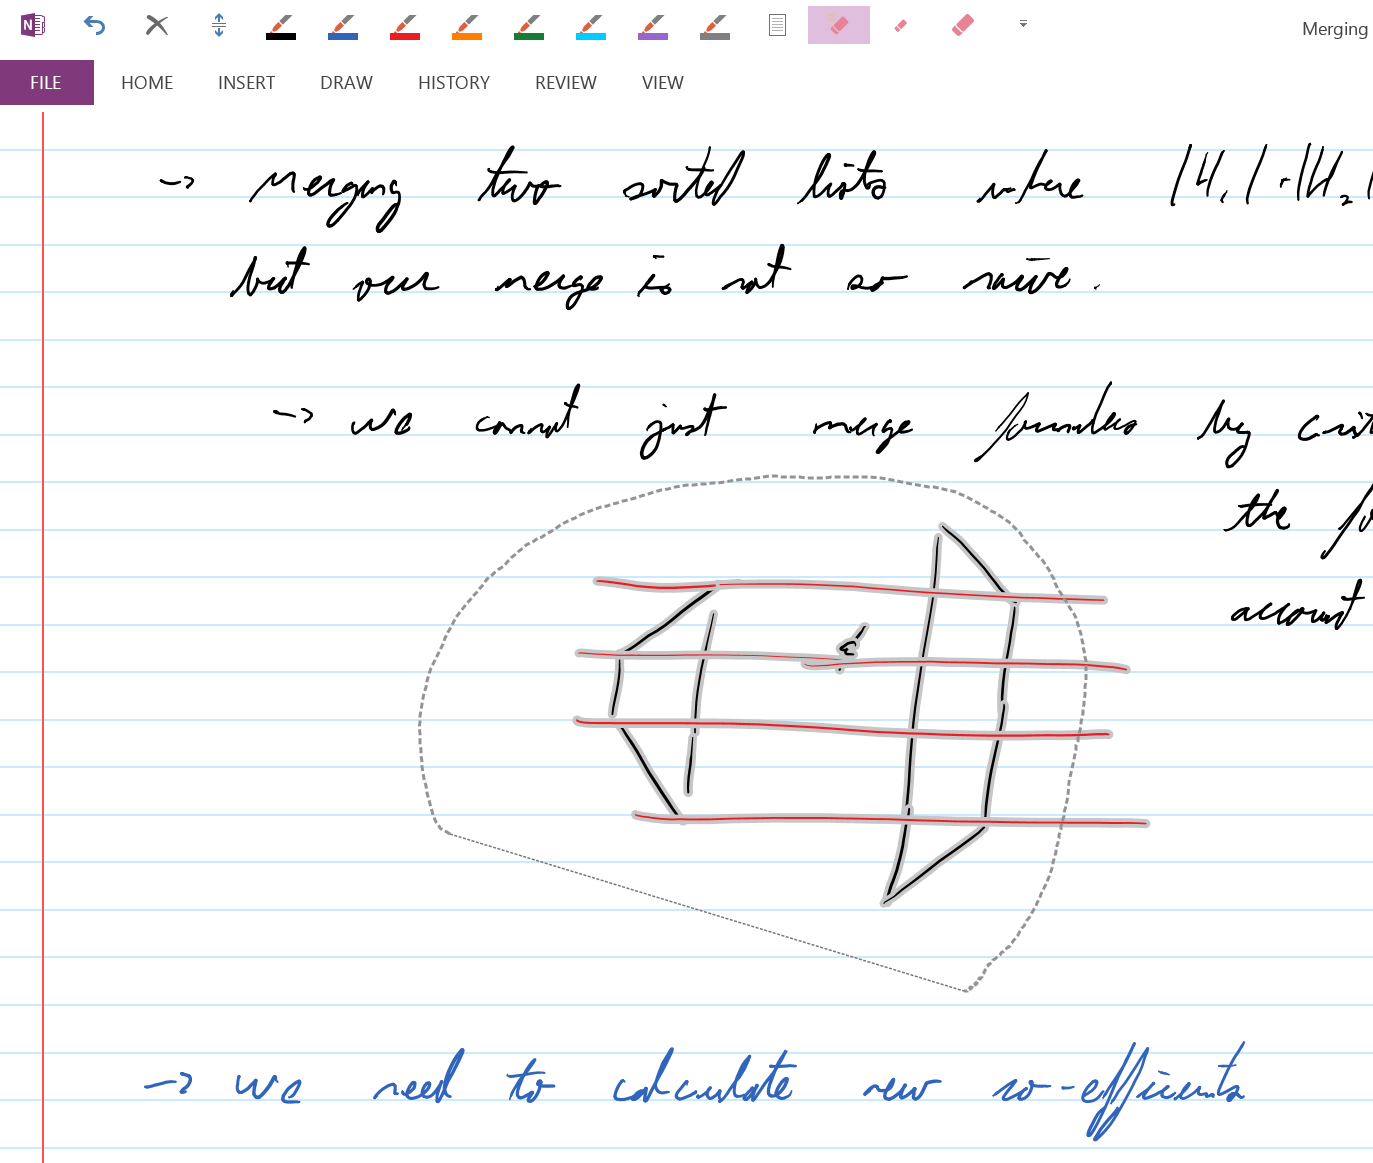
\includegraphics[width=0.50\textwidth]{figures/fig_onenote}
  \caption[An example of practical partial enclosure range searching]{An example of practical partial enclosure range searching in Microsoft OneNote. The line segments in the middle are selected even though they are not entirely enclosed.}
  \label{fig:intro:onenote}
\end{center}
\end{figure}

Looking carefully at the figure, we can see that even though the horizontal line segments of the diagram have not been entirely enclosed by the selection tool, they nevertheless appear as part of the set of selected items.
This behaviour of selecting partially enclosed objects is described in a patent filed by Microsoft Corporation\cite{lassoselect}. 
From the patent:

\begin{quote}
[T]here is a need for a selection tool that will allow a user to conveniently select one or more graphical objects in their entirety, without requiring an inconvenient amount of precision from the user.
\end{quote}

\noindent With the rising popularity of touch and pen-enabled devices, this need is likely to increase.  
As we can see from the figure, OneNote already includes an implementation of a partial selection tool like the one described by the patent. 
Although the details of the implementation are proprietary, it becomes apparent while using the software that it suffers from poor performance as more items are selected.
It is from this observation that the work in this thesis was inspired.  
Although the problems that we will examine take place in simpler settings than the patent describes, we will nevertheless develop an understanding of the major challenges of this problem domain, as well as some techniques for addressing them.


%------------------------------------------------------------------------------
%------------------------------------------------------------------------------
\section{Problem Statements}
\label{:intro:problems}

This thesis proposes algorithms for several different partial enclosure range search settings.  Each problem addresses a different type of geometric object to be queried, or a different type of query region.

\paragraph{Line Segments and Query Rectangles.} Line segments and rectangles are one of the simplest settings in which we can perform partial enclosure range searches. 
Given an axis-parallel query rectangle, we address methods which consider only axis-parallel segments, or which consider arbitrarily-oriented ones.

\paragraph{Line Segments and Query Slabs.} Relaxing the axis-parallel query regions of the preceding problem, we consider an arbitrarily-oriented slab.
As the query slab can have any orientation, intersections with a horizontal segment will involve both the height of the segment and the slope of the slab.  
We also consider a query defined as the intersection of two slabs.

\paragraph{Convex Polygons and Query Rectangles.} Moving away from line segments, we consider problems of partial enclosure with respect to area.  
For any such problem, deciding on the partial enclosure property is straight-forward once we know the area of the input object and the area enclosed by a query region.  
We consider how to determine what proportion of a convex polygon is enclosed by a rectangular query.
 
\paragraph{Monotone Polygons and Query Rectangles.} This more complex shape does not generally decompose into big convex regions, so a different method of preprocessing will be needed.
We consider methods for calculating the area of the polygon to one side of a query line. 
With such a method in hand, determining the area of a rectangle is a matter of executing several queries and combining their results.

%------------------------------------------------------------------------------
%------------------------------------------------------------------------------
\section{Related Work}
\label{:intro:related}

In this section, we review some existing variations of the range searching problem.
As a whole, due to its applicability to such a wide assortment of problems, range searching has received a great deal of research attention.
Aside from the solutions to specific problems that this research has found, it has also resulted in a vast toolbox of observations and techniques, many of which apply to our own problem.

Range searching structures are typically constructed by subdividing the input objects, or the space in which the input objects exist, into several regions which express helpful properties.
Ideally, we are able to choose these regions so that a query region will entirely contain, or not contain, most of the regions, while intersecting only a small number of them.
On those intersected regions, we continue the query on the recursively finer subdivisions stored there.\cite{Matousek93}

This recursive decomposition of the input into regions has an extremely beneficial side-effect. 
At each hierarchical regions, we must associate the further decomposition of the regions, but we can associate other structures as well.
These so-called multi-level structures can be used to answer complex queries by identifying objects which satisfy one property, and then continuing the query on the associated structures to satisfy additional properties.
We discuss examples of this type of multi-level query in detail in Chapter~\ref{:prelim}.

The remainder of this section gives a brief introduction to some specific range search problems, and some methods for answering each. 
We refer the reader to an excellent survey on range searching by Agarwal and Erickson\cite{Agarwal99} for a more detailed introduction.


\subsection*{Orthogonal Range Searching} 

In its general form, an orthogonal range searching problem starts with a set $S$ of points in $\mathbb{R}^d$, where $d$ is a small, fixed constant.
A query is a $d$-dimensional, axis-parallel box, and our goal is to identify the subset of our input points which are contained within this box.

\emph{Quadtrees} were first described by Finkel and Bentley\cite{Finkel74} (see also \cite{debergch14}) and are one of the very first structures for performing range searches.
When we are considering points in the plane, a quadtree works by dividing the space into squares, and then recursively splitting any region which contains more than one point into four smaller, but equally-sized squares.
Because this recursion is based on splitting space rather than the points within the space, the recursion depth, and thus the depth of the quadtree, is not related to the number of points. 
Instead, the size of the initial square from which we start splitting and the distance between the closest pair of points are the important factors.
For an initial square with a side length of $s$ and a closest pair with distance $c$, the recursion depth is $\BigOh{\log{\frac{s}{c}} + \frac{3}{2}}$.
The construction and query times are related to this recursion depth, making the structure somewhat slow, but it \emph{does} work!
Quadtrees can also be extended to work in higher dimensions easily enough. 
In $\mathbb{R}^3$ quadtrees are instead called \emph{Octrees}, and the general method can be extended to even higher dimensions. 
For points and an initial box in $\mathbb{R}^d$, decomposition proceeds along the same basic rules, but using progressively smaller $d$-boxes instead of just squares.


KD-Trees\cite{Bentley75} were the first major improvement over quadtrees.
Unlike a quadtree which partitions space, a KD-Tree directly partitions the pointset in a recursive manner.
For points in the plane, each level of the tree corresponds to a particular axis.
Suppose that we start with the $x$-axis at the root level.
We consider the median point $m$ with respect to the $x$-coordinates of all the points, and then all remaining points are partitioned as left or right of this vertical \emph{splitting line} through $m$.

On the next level of the recursion we alternate to the $y$-axis, select the median point with respect to their $y$-coordinates, and partition around the horizontal splitting line through that point.
The process continues, alternating the axis on each level, until we create leaves containing single points.

This process creates a balanced tree, where each path through the tree alternates between axes.
Each node in the tree represents a region of the plane bounded by its own splitting line and the splitting lines of its ancestors.

Querying a KD-Tree by a rectangular region involves traversing the tree while only visiting those nodes where their region is intersected by the query region.
While the preprocessing requirements of a KD-Tree are quite good, at $\BigOh{n}$ space and $\BigOh{n\log{n}}$ preprocessing time, the query time is $\BigOh{\sqrt{n}}$.

A final note about KD-trees, this recursive construction can be generalized to higher dimensions in a straight-forward manner, by simply cycling through each of the $d$ axes in order.
The preprocessing requirements are unchanged asymptotically, since we still create just a single binary tree with $n$ leaves.
The query algorithm is also similar to the $\mathbb{R}^2$ case, but with a query time of $\BigOh{n^{1-1/d}}$.

The next improvement in orthogonal range searching came in the form of a polylogarithmic method known as \emph{Range Trees}. 
This method was discovered by Bentley\cite{Bentley79}, who was involved in the last two structures, but  were also simultaneously developed by independent researchers.
This method is constructed on binary search trees and can query any open or closed query box in $\BigOh{\log^{d-1}{n}}$ time with only $\BigOh{\log^{d-1}{n}}$ time and space pre-processing.
We discuss this structure in more detail in Section~\ref{:prelim:range-trees}.

%Best known by Chazelle [Dutch 90,91] in 2D and higher dimensions with time/space of XXX

Finally, a noteworthy special case occurs when our points are in the plane and our query is a three-sided rectangle, i.e., when it is open to one side.
In this case, we can use a method developed by McCreight\cite{McCreight85} which gives $\BigOh{\log{n}}$ query time while using only $\BigOh{n}$ space and $\BigOh{n\log{n}}$ preprocessing time.

The real power of orthogonal range searching is in how other problems can be reduced to instances of it by encoding query keys as coordinates of a high-dimensional point.  
For example, in the geometric sense, we can search for rectangles inside of rectangles by mapping the coordinates of an input rectangle in $\mathcal{R}^{d}$ to a point in $\mathcal{R}^{2d}$, and performing an orthogonal range search in that space.
Rectangle-in-rectangle queries are important as rectangles make easy approximations of more complicated geometric objects that we may want to look for.

Outside of purely geometric applications, many more general types of range searching problems can be reduced to instances of orthogonal range searching by encoding query keys as coordinates of a high-dimensional point.
For example, given some integer representation of a date, we can search for emails received within a date range by encoding the date stamp of each email into a point, and then searching for points between the two integer representations of our query range.
Extending this idea to more complex queries is just a matter of mapping each key we wish to search on to further components of a higher-dimensional point.  
In this way, multi-dimensional orthogonal range searching can be used to perform multi-key searching.\cite{Willard96} 


\subsection*{Half-plane Range Searching}

History

Lower bounds;  
Half-planar searches cannot be done in near linear space with polylogarithmic query time, meaning that we will have to decide which we want more, low space or low query time, when choosing a structure for a problem at hand.
We introduce a structure suitable for each side of this trade-off.

If we want to save space, we can use a \emph{Ham Sandwich Cut Tree}\cite{Edelsbrunner86, Edelsbrunner87}.
To produce a ham sandwich cut tree, we divide all of our points into four quadrants of equal size, which we accomplish with an algorithm by Megiddo\cite{Megiddo85} in $\BigOh{n}$ time.
We continue by repeating this construction on each quadrant recursively, and constructing a tree.
This tree contains each point as a leaf, and recurses on a constant fraction of the points at each step, so the result is a tree of size $\BigOh{n}$ constructed in $\BigOh{n\log{n}}$ time.

We can query this tree with the line representing the boundary of our half-plane.
The quadrants at any step are the result of two intersecting lines, and thus, our query line will intersect at most three of them.
The non-intersected quadrants, of which there is at least one, are entire entirely inside the half-plane bordered by the query line, or entirely outside of it.
The query then recurses on the intersected quadrants.
Total query time is $\BigOh{n^{\log_2(1 + \sqrt{5}) - 1}} \approx \BigOh{n^{0.695}}$.

If we want to save query time, then we can use a \emph{Level Arrangement}.  
This structure has a query time of only $\BigOh{\log{n}}$, but requires $\BigOh{n^2}$ storage.
The level arrangement structure is constructed on the dual lines corresponding to each point.
That is, given a set $S$ of $n$ points $p_1, p_2, \ldots, p_n$ where each $p_i = (a_i, b_i)$, we map each point to a corresponding line $l_i: y = a_i \cdot x + b_i$.

When we consider all of the intersection points and edges formed by the set of dual lines, our arrangement has size $\BigOh{n^2}$.
By checking the intersections of the lines, we can enclose the ``interesting'' part of the environment inside a bounding box.
From here, we construct envelops.

In this dual space, the query line which defines the boundary to a half-plane becomes mapped to a point, and the original point satisfying the half-plane correspond to the levels which are found above or below the point in the arrangement.

What is the remainder of the construction? How does the query proceed?

Finally, when we consider a half-plane as a degenerate simplex, this type of query can also be answered by the structure we discuss in Section~\ref{:prelim:chan}.


\subsection*{Simplex Range Searching}

When we leave axis-parallel boxes behind, we move into arbitrary simplices and half-spaces, which can be thought of as degenerate simplices.

In $\mathbb{R}^2$, we get half-planes when we look for everything to one side of a line, or, for closed regions, a triangle.

There is no known data structure which can answer a simplex range search in polylogarithmic time using near linear storage, and the lower bounds which have been discovered for this problem leave us looking for tradeoffs.\cite{Agarwal99}

If we would like to save space and spend more time on queries, then we will probably use a partition tree approach, as introduced by Willard~\cite{Willard82}. 
His method is specifically for points in the plane and expresses the ``nice'' recursive structure idea we mentioned above by exploiting the Ham Sandwich cut theorem~\cite{XXX}.
His result requires query time of $\BigOh{n^{\log_3{4}}}$.
This was improved by \cite{EW} to approximately $\BigOh{n^{0.695}}$.

As the partition tree approach is most concerned with how many partitions are intersected by a query, as opposed to those partitions which are entirely to one side of a query, understanding the \emph{crossing number} of a set of partitions is key to reducing the query time.
Welzl\cite{W} was able to develop a partitioning method with a crossing number of $\BigOh{n^{1-1/d}\log{n}}$, and later, Chazelle and Welzl\cite{CW} got this number down to just $\BigOh{n^{1-1/d}}$.
In the plane, this gives us roughly $\BigOh{\sqrt{n}}$ query time for $d \leq 2$, but does not extend to $d \geq 3$.

If we would like to have a logarithmic query time.


\subsection*{Intersection Searching} 

Intersection searching is similar to range searching, except that we consider different types of geometric input objects aside from points.
Given a query range, we are looking for any objects which have even a single point of intersection in common with the query itself.
In this way, we can think of range searching as a specialization of intersection searching.

In \emph{Segment Intersection Searching}, the query range is a line segment. 
If both the input objects and the query range are segments, 

\emph{Rectangle Intersection Searching}, also known as \emph{Windowing Queries} identify polygons which intersect a rectangular query region. 
Many computer graphics problems are related to this problem as, for example, we might want to determine what items need to be rendered on screen from a 3D environment.

Finally, \emph{Point Intersection Searching} is sort of the opposite of an normal range searching query. In this problem, we are interested in reporting all objects which contain a query point.


\subsection*{Completing a Search}

Throughout this section, we've used the term ``identify'' rather loosely.
For the hierarchical structures above, ``identifying'' points satisfying a query really comes down to isolating those partitions which contain them.
What we do with them at that point is somewhat flexible.
For example, we can simply count the points we have identified with only a constant factor of extra time and space by having the partitions store their own sizes.
We could instead report the points by traversing each terminal of the partition, which will cost us an extra linear factor with respect to to the number of reported items.

Our problem is notably different from standard range searching problems because we are not just looking for items which are entirely contained inside of a query region.
This immediately rules out a simple application of orthogonal range searching like we saw with the rectangles-in-rectangles problems.

Our problem differs from intersection searching as well, since we have the extra constraint of requiring a specific proportion of the input objects to be contained in the query region, rather than just any point.


%------------------------------------------------------------------------------
%------------------------------------------------------------------------------
\section{Summary of Contributions}
\label{:intro:contributions}

In this thesis, we develop contributions to several variations of the \PERS{} problem, along with some noteworthy ancillary methods. 
Table~\ref{tab:contributions} gives a broad overview of the data structures we develop. 
The table uses `AP' for ``Axis-Parallel'', `AO' for ``Arbitrary Orientation'', and `P' for ``Polygon'', and omits ``Big Oh'' for clarity.

\begin{table}[t]
\caption{Summary of Contributions}
\label{tab:contributions}
\centering
\begin{tabular}{l l l l l l}
\hline \hline
Object & Query & Theorem & Space & Time & Query \\
\hline
AP Segment & AP Rectangle & Th~\ref{th:ap} & ${n\log^3{n}}$ & ${n\log^3{n}}$ & ${\log^3{n}}$ \\
AO Segment & AP Rectangle & Th~\ref{th:ao} & ${n\log^7{n}}$ & ${n\log^7{n}}$ & ${\sqrt{n}\log^7{n}}$ \\
AP Segment & AO Slab & Th~\ref{th:slabs:one} & ${n\log^2{n}}$ & ${n\log^3{n}}$ & ${\sqrt{n}\log^3{n}}$ \\
AP Segment & 2 AO Slabs & Th~\ref{th:slabs:two} & ${n\log^3{n}}$ & ${n\log^3{n}}$ & ${\sqrt{n}\log^3{n}}$ \\
Convex P & Rectangle & Th~\ref{th:convexp:area} & ${n}$ & ${n}$ & ${\log{n}}$ \\
Convex P & Convex $k$-gon & Cor~\ref{cor:convexp:karea} & ${n}$ & ${n}$ & ${k \log{n}}$ \\
Monotone P & AP Rectangle & Th~\ref{th:monotonep:rect:area} & ${n\log{n}}$ & ${n\log{n}}$ & ${\log{n}}$ \\
Monotone P & AP Rectangle & Th~\ref{th:mono2} & ${n}$ & ${n\log{n}}$ & ${\sqrt{n}}$ \\
Simple P & Horiz Slab & Cor~\ref{cor:monotonep:simplep-area} & ${n}$ & ${n}$ & ${\log{n}}$ \\
\hline
\end{tabular}
\end{table}

In the line segment cases, we develop methods for restating the partial enclosure property as something which can be evaluated as a one or two variable inequality. 
These expressions can then be queried by known structures for orthogonal or half-plane queries. 
We discuss the transformations to appropriate dual-spaces and the design of data structures which can answer the necessary multi-part queries.

In the polygon cases, we primarily develop methods for calculating area within a simple region, e.g., below a query line.
These methods are then repeated and combined to find the area enclosed by the actual query region.
Once the enclosed area is known, determining the partial enclosure property is straight-forward.

%------------------------------------------------------------------------------
%------------------------------------------------------------------------------
\section{Organization of the Thesis}
\label{:intro:organization}

The remainder of this thesis is organized in the following way. 
Chapter~\ref{:prelim} reviews existing data structures and range searching techniques which we utilize in our own contributions.
The next four chapters cover partial enclosure range searching queries on successively more sophisticated geometric objects, with Chapter~\ref{:rectangles} focusing on axis-parallel rectangles, Chapter~\ref{:slabs} on arbitrarily-oriented slabs, Chapter~\ref{:convexp} on convex polygons, and Chapter~\ref{:monotonep} on monotone polygons.
The thesis concludes with Chapter~\ref{:conclusion} which summarizes the contributions and future work presented in earlier chapters.
